\chapter{Literature Review}
\section{Introduction}
The first reported cases of COVID-19 occurred in Wuhan, China on December 12th, 2019\cite{CDCCovidTimeline}, when a number of patients began to exhibit ''symptoms of an atypical pneumonia-like illness that does not respond well to standard treatments''.  It was not until December 31, 2019, that the World Health Organization(WHO) Country Office in China was informed of several more cases of this strange virus described as ''pneumonia of unknown etiology'', the symptoms of this new virus were shortness of breath and fever.  All the initial cases observed seem to have been connected to a market called Huanan Seafood Wholesale Market.  On January 1st of 2020, the Huanan Seafood Wholesale Market was shut down amid concerns over the spread of this new virus.  On January 3rd the Government of China alerted the World Health Organization that they had identified over 40 new cases of this pneumonia-like disease, and on the 5th of January, Chinese public health officials shared the genetic sequence of the new virus with the world through a database that could be accessed by the public.  Following the release of this information the CDC (Centers for Disease Control and Prevention), which is a US Government funded healthcare research agency, began an investigation into the origins of this new virus.  The origins of COVID-19 are not clear and are still being researched.  The most likely explanation offered by scientists is that it originated in the Huanan Seafood Wholesale Market from animals sold there - a likely culprit is the Raccoon Dog which is used for fur and food in China\cite{CovidOriginsMarket}, but other theories suggest that a lab leak at a biological weapons facility\cite{CovidOriginsLab} may be responsible for the creation of the virus.  Some researchers are currently suggesting that blood samples taken from animals sold at the Hunan Market and samples from the people who sold them may lead to definitive evidence of the disease's origins\cite{CovidOriginsMarket}.
\\
Although the origins of COVID-19 still remain up for debate it is clear that when studying the virus, its high transmission rate and the speed at which it can spread made it one of the deadliest viruses in human history.\cite{smithsonianCovid191918Flu}\cite{nationalGeographicCovid191918Flu}
\begin{figure}[H]
    \centering
    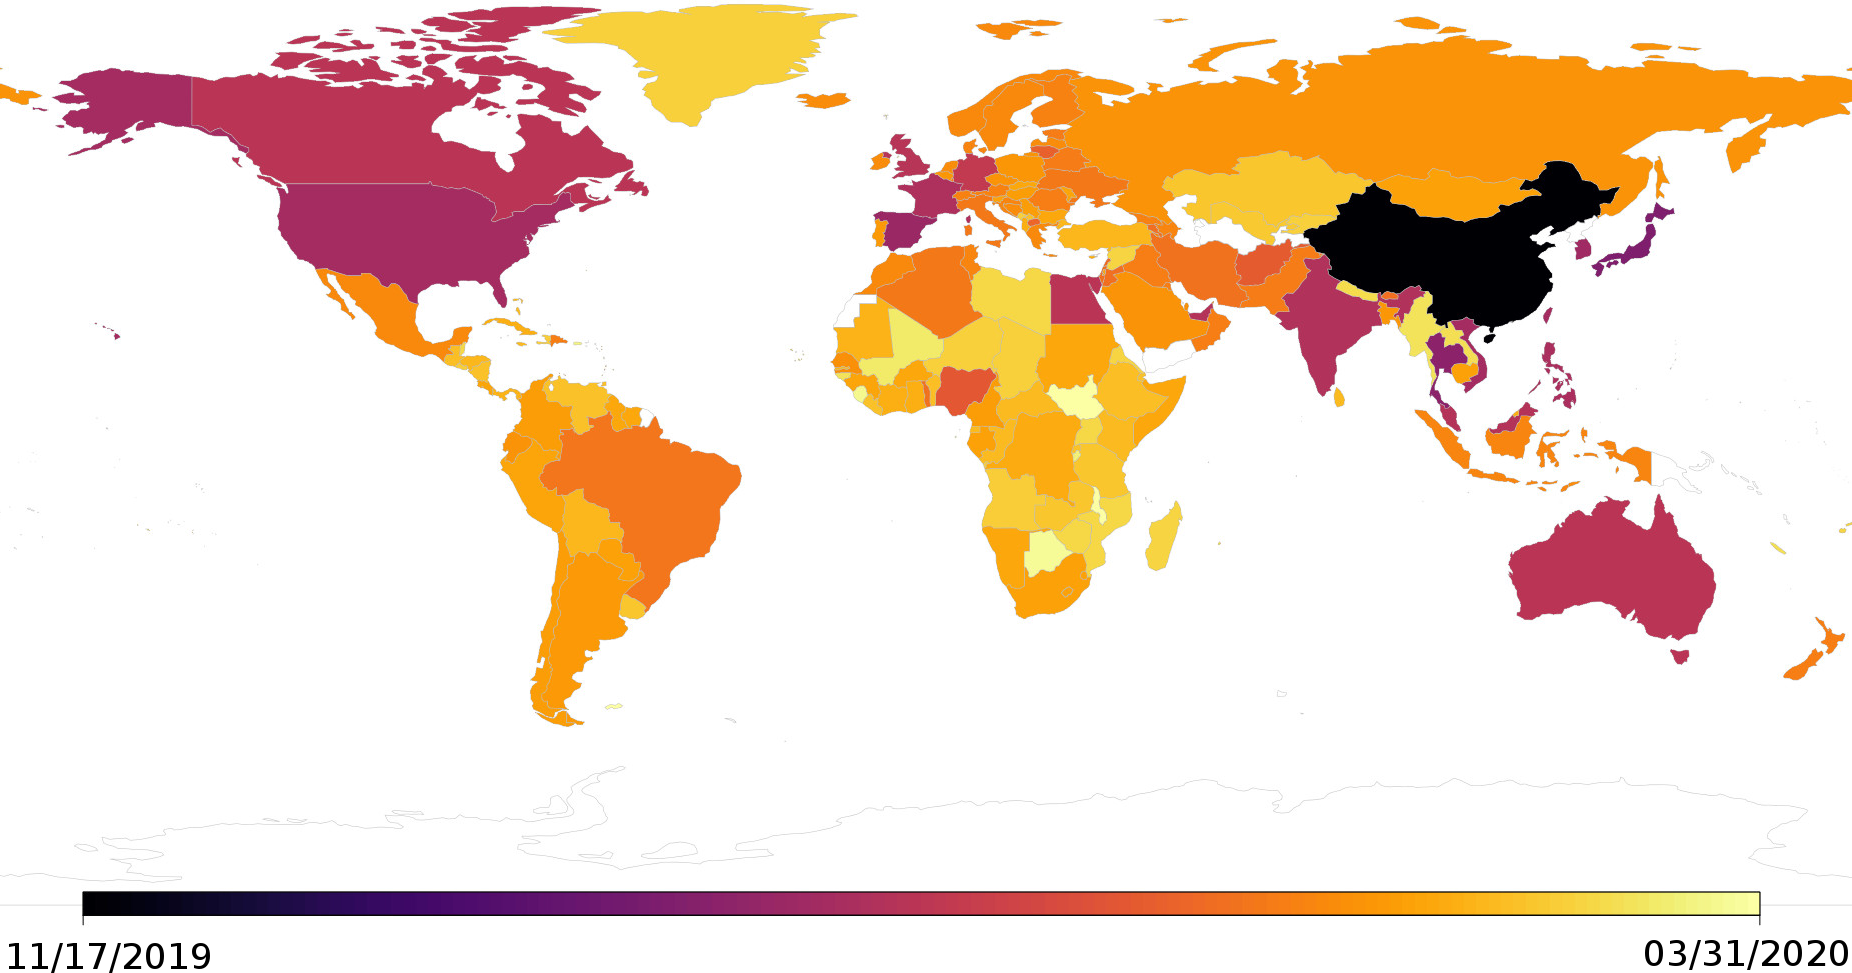
\includegraphics[width=1\textwidth,keepaspectratio]{Images/DateOfFirstCovidCaseMap.png}\\
    \caption{Estimated dates of first COVID-19 cases around the World, Image courtesy of Roberts, Rossman and Jarić\cite{covid19SpreadMap}}
    \label{fig:COVID-19 Case Map}
\end{figure}
\vspace{0.5mm}

Due to this rapid spread of the virus, many governments were unprepared for dealing with such an outbreak.  The artificial intelligence community had published many papers and conducted much research into designing automated tools which could relieve medical professionals of the extreme stress they were under. Unfortunately, most of the models trained were of no use to medical professionals and some were even deemed harmful\cite{mitTechReviewCovid19}.    There were many limitations when it came to training automated diagnostic tools for COVID-19, such as incorrect assumptions about the data, lack of data quality, and lack of data in general.  Due to the poor / limited quality of data and the urgent need for diagnostic tools, many of the models were trained using poor-quality data or incorrect data.  Such poor models would have had drastic effects if patients who were COVID positive were diagnosed as negative by the model, and models suffering from high false negative rates would have drastic consequences for the patients afflicted with COVID.
\\
The models trained on what have been termed as ''Frankenstein Datasets'' suffered immensely, as some of the data came from the same source, meaning the same data from the training set could have been present in the test set. This would severely impact the performance of the model, as it would have to overfit the data from which it was trained.  These models which were overfitted on the data would seem to have high accuracy but ultimately would perform poorly on real-world data.
 \begin{figure}[H]
    \centering
    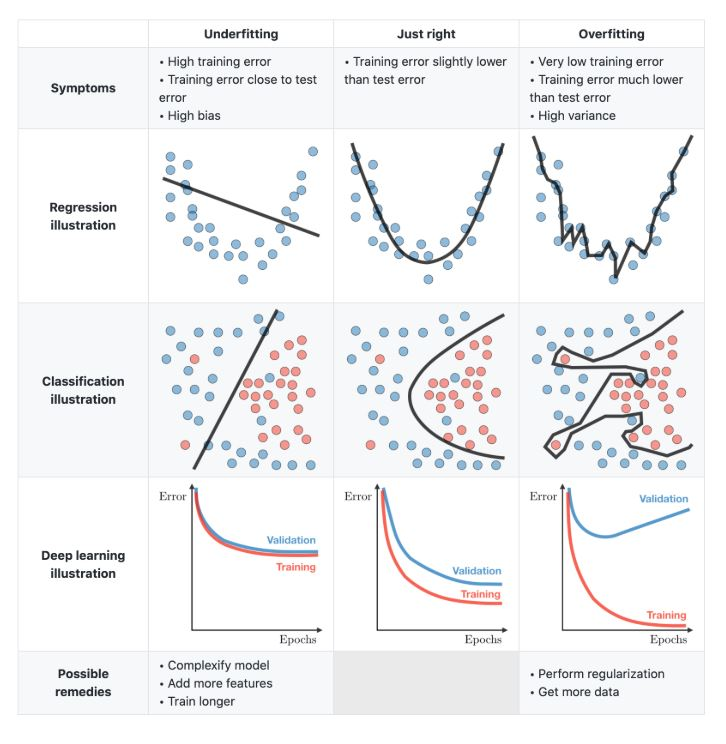
\includegraphics[width=1\textwidth,height=13cm,keepaspectratio]{Images/OverfittingUnderfitting.png}\\
    \caption{Examples of Overfitting, Underfitting and Optimal models, Image courtesy of Abhishek Shrivastava\cite{overfittingKaggle}}
    \label{fig:Examples of Overfitting, Underfitting and optimal models}
\end{figure}
\vspace{0.5mm}
Figure \ref{fig:Examples of Overfitting, Underfitting and optimal models} above shows how a model's performance can be analyzed. Underfitting yields a high training error and high bias meaning that the model will perform poorly on the training, test, and dev sets.  Overfitting leads to a very low training error which will be lower than the test, and dev set error and wouldn't be fit for purpose when analyzing real-world data.   The optimal model has a training error that is slightly lower or in and around the same accuracy as the test and dev sets.
\\
The lack of medical experience also played a role in the poor performance of these models as many of the AI researchers training these models would be unfamiliar with flaws in the data.  The bias of the radiologist labeling the X-rays of patients also played a role as the radiologist could have inaccurately diagnosed the patient as COVID positive or negative.  Private Artificial Intelligence companies also played a role in poor model development as published models from researchers tied to the company also showed that these models had a high risk of bias.\cite{mitTechReviewCovid19}
\\
As the pandemic progressed more and more data was made available to researchers which was able to mitigate some of the problems stated above, leading to more accurate and robust models which we will explore in the later sections.
\section{Analysis of Existing Models for Automated COVID-19 Detection}
In a paper by Mahmoudi, Benameur et al \cite{litReviewDeepLearningCovid19} researchers investigated a deep-learning approach to creating a diagnostic tool for COVID-19.  The research involved utilizing data taken from computed topography scans.  These scans segmented the infected regions of a patient's lungs to determine if said patient was afflicted with the COVID-19 virus.  The researchers also used a technique called "Contrast Limited Adaptive Histogram Equalization" which is a preprocessing method that removes noise and intensity to create a homogeneous dataset.  The researchers also removed black slices from the images so that only the region of interest was highlighted, with the goal of further improvement of the performance of the model.  U-Net architecture is an architecture that is based on convolutional neural network encoders and decoders, this architecture was used in the creation of this model to allow for more timely and accurate segmentation of images and to generate the segmentation models of the lung and infection x-rays.  Four-fold cross-validation (this is where the dataset is sliced into four equal parts depending on the size for odd datasets there may be set with the remainder of values if not equally divisible by four), then the models are trained on one or multiple sections, and tested with another section. The final model is taken from the model with the best performance and was then used to analyze the performance of the model along with a three-layered CNN architecture which was comprised of added fully-connected layers which was connected to a softmax output layer, the output layer was used for classification of the images. 
 \begin{figure}[H]
    \centering
    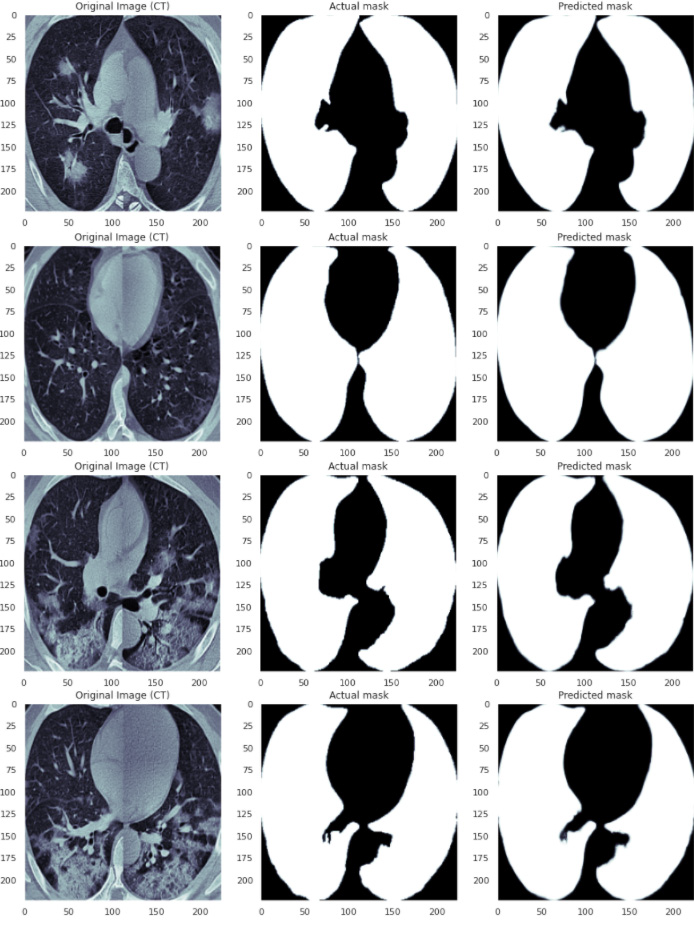
\includegraphics[width=1\textwidth,height=15cm,keepaspectratio]{Images/CTScanQualitativeImage1.png}\\
    \caption{Examples of CT Qualitative images lung segmentation\cite{litReviewDeepLearningCovid19}}
    \label{fig:Examples of CT Qualitative images lung segmentation}
\end{figure}
\vspace{0.5mm}
 \begin{figure}[H]
    \centering
    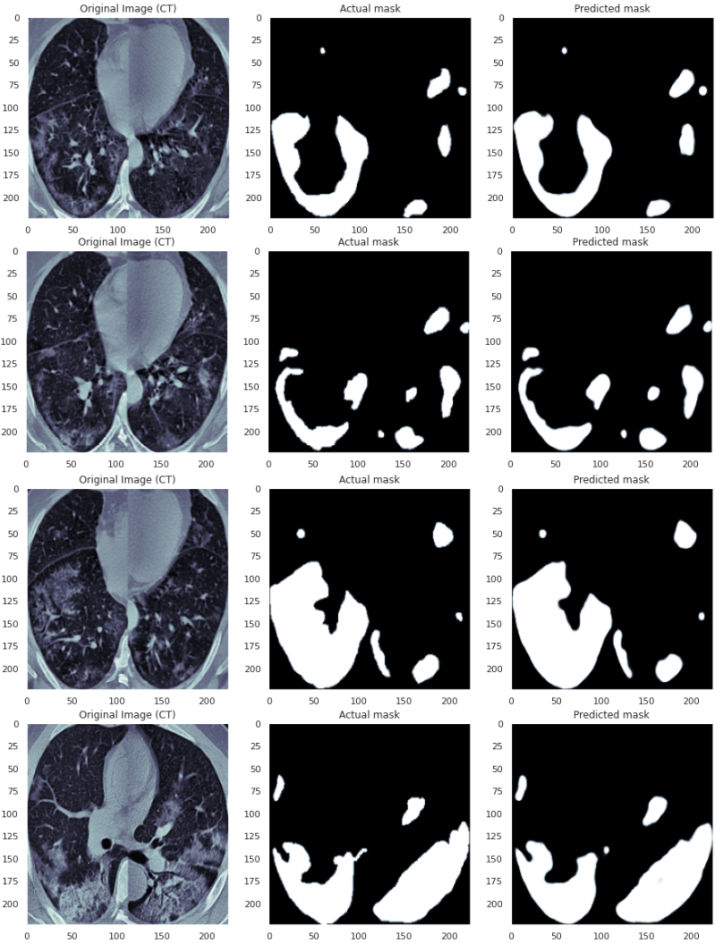
\includegraphics[width=1\textwidth,height=15cm,keepaspectratio]{Images/CTScanQualitativeImage2.png}\\
    \caption{Examples of CT qualitative images infection masks\cite{litReviewDeepLearningCovid19}}
    \label{fig:Examples of CT qualitative images infection masks}
\end{figure}
\vspace{0.5mm}
Figure\ref{fig:Examples of CT Qualitative images lung segmentation} shows the lung segmentation results, one column containing the ground truth and the other containing the researchers' proposed four slice model, which is compromised of four slices taken from different CT scans.  The first column shows the original CT scan, the second column shows ground truth, and finally, the third column shows predicted lung masks.
\\
Figure \ref{fig:Examples of CT qualitative images infection masks} we can observe the qualitative comparison between the researchers' infection segmentation results which is made up of four slices from different CT scans and the ground truth. The first column shows the original CT scan, the second column shows the ground truth, and finally, the third column shows predicted infection masks
\\
Utilizing a 70\% - 30\% training set and validation set split, the researchers were able to demonstrate that the system proposed attained a dice score (a value ranging from 0 - 1, used to gauge performance by comparing the results of the output of the model to that of the ground truth, where 1 is a perfect overlap and 0 is no overlap) of 98\% and 91\% for lung and infection segmentation tasks.  Additionally, the system accurately diagnosed patients afflicted with COVID-19 98\% of the time.  The development of this model suffered from a lack of data, as only 20 CT scans were used to train and test the model. The limited data set used suggests the researcher's model may have possibly been overfitting the training data.  The researchers mention as much in the conclusion section of this paper. They discuss how the main limitation of the study is the use of a small but sufficient amount of training data.  The restrictions on data collection coupled with the high cost of labelling the data meant that the researchers were only able to utilize the 20 CT scans for both training and testing the model. From the conclusion section of this paper, it is clear that there is a high potential for bias in the data set used by the researchers.  The possibly mislabelled images links back to the ''Frankenstein Datasets'' which I mentioned in the introduction section of this literature review.
\\
In another paper by Islam, Islam, and Asraf\cite{litReviewCnnLstm} we see a new method being used by researchers to develop an automated diagnostic tool.  The researchers used a combination of a convolutional neural network with LSTM (long short-term memory), they used the convolutional neural network for deep feature extraction and LSTM for detection of COVID-19 using an extracted feature.  They also used a dataset containing 4575 X-ray images which included 1525 images of COVID-19 X-rays.  The experimental results of the system are as follows: 99.4\% accuracy, AUC (area under curve) accuracy of 99.9\%, specificity of 99.2\%, sensitivity of 99.3\% , and finally an F1 score of 98.9\%.  The researchers suggest that this system could be further improved in the abstract if more data were available to the researchers.  As we can see this study also appears to suffer from a lack of data as per the previous paper discussed.  The lack of data is clearly visible but by utilizing an LSTM network the researchers further improved upon the diagnostic model discussed in the previous paper by Mahmoudi et al.  The dataset used was also greater in size than the dataset used in the prior paper, this would lead to a more robust model with a greater ability to generalize.
\vspace{0.5mm}
 \begin{figure}[H]
    \centering
    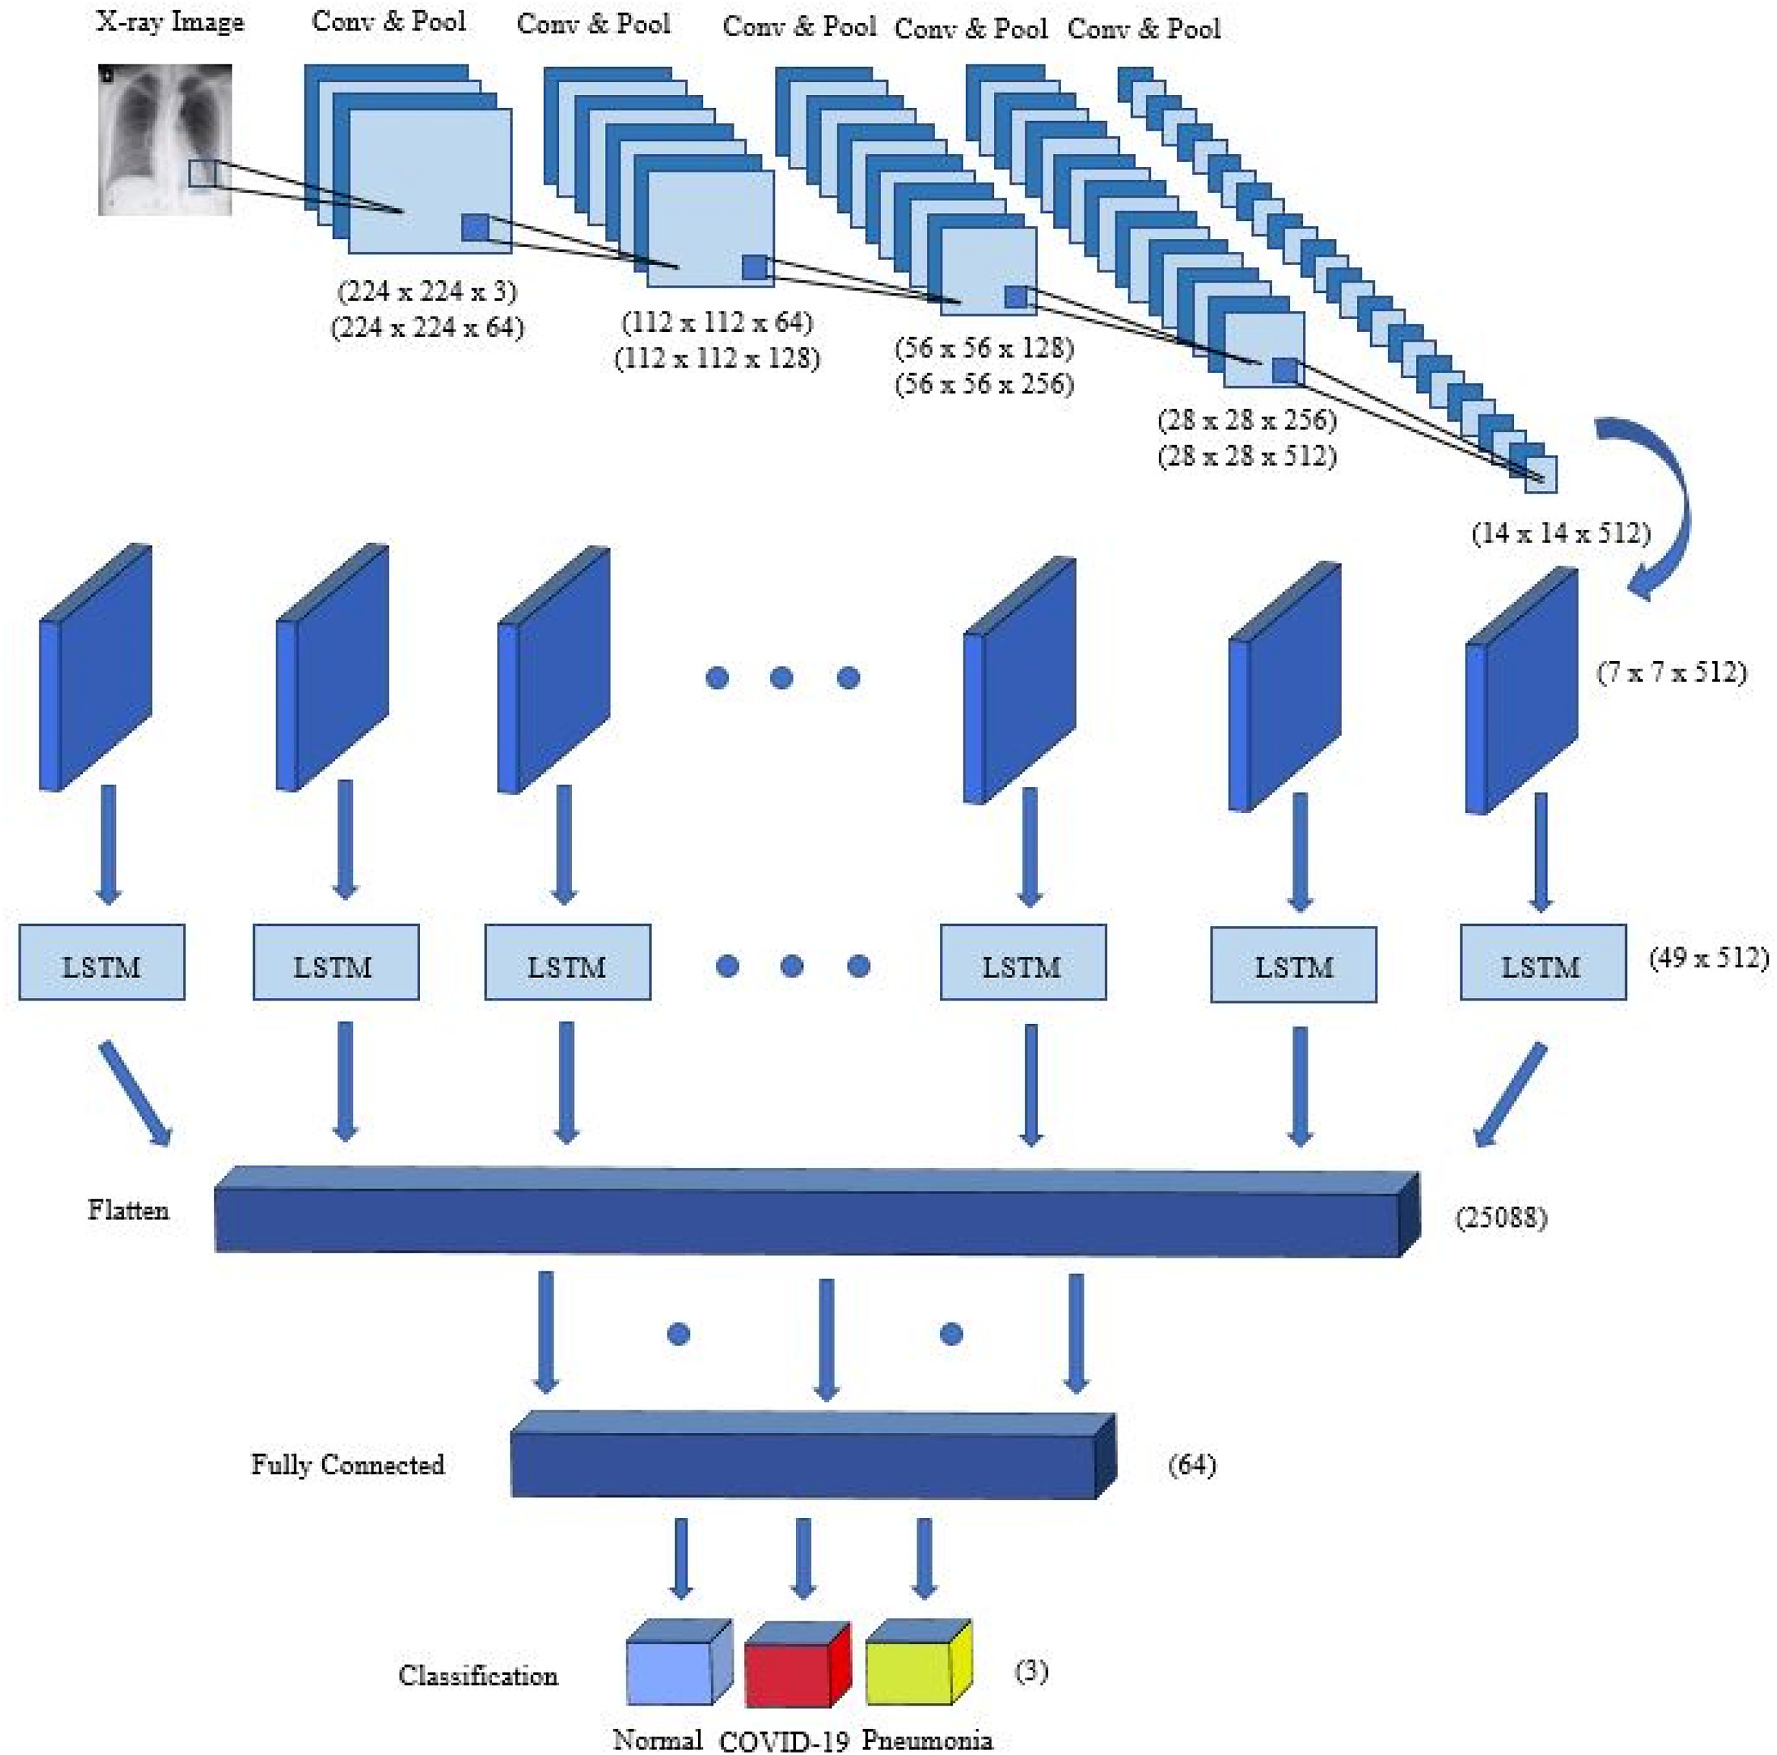
\includegraphics[width=1\textwidth,height=10cm,keepaspectratio]{Images/lstmDiagram.png}\\
    \caption{Overview of a Typical LSTM Network\cite{litReviewCnnLstm}}
    \label{fig:Diagram of Long Short Term Memory Network}
\end{figure}
\vspace{0.5mm}
The model benefited from the use of LSTM, as an LSTM network has an internal memory that is utilized to learn from experience with long-term states. LSTM is based on recurrent neural networks, and improves upon them by using memory blocks instead of conventional RNN units, this helps to solve the vanishing and exploding gradient problem\cite{vanishingExplodingGradients}.  In addition to the memory blocks, there is also a cell state which saves long-term states, the cell states being the main difference between recurrent neural networks and LSTM.  The network is capable of remembering and connecting previous information to present data\cite{lstmRemembering}.  The LSTM Network is comprised of three gates the input gate which is termed the ''forget gate'', an update gate, and finally an output gate.  These gates essentially determine which data is worth remembering and which data can be forgotten.
\\
The results achieved by the various models are shown in figure \ref{fig:Performance of CNN Model Literature Review} and figure \ref{fig:Performance of CNN LSTM Model Literature Review}

\vspace{0.5mm}
 \begin{figure}[H]
    \centering
    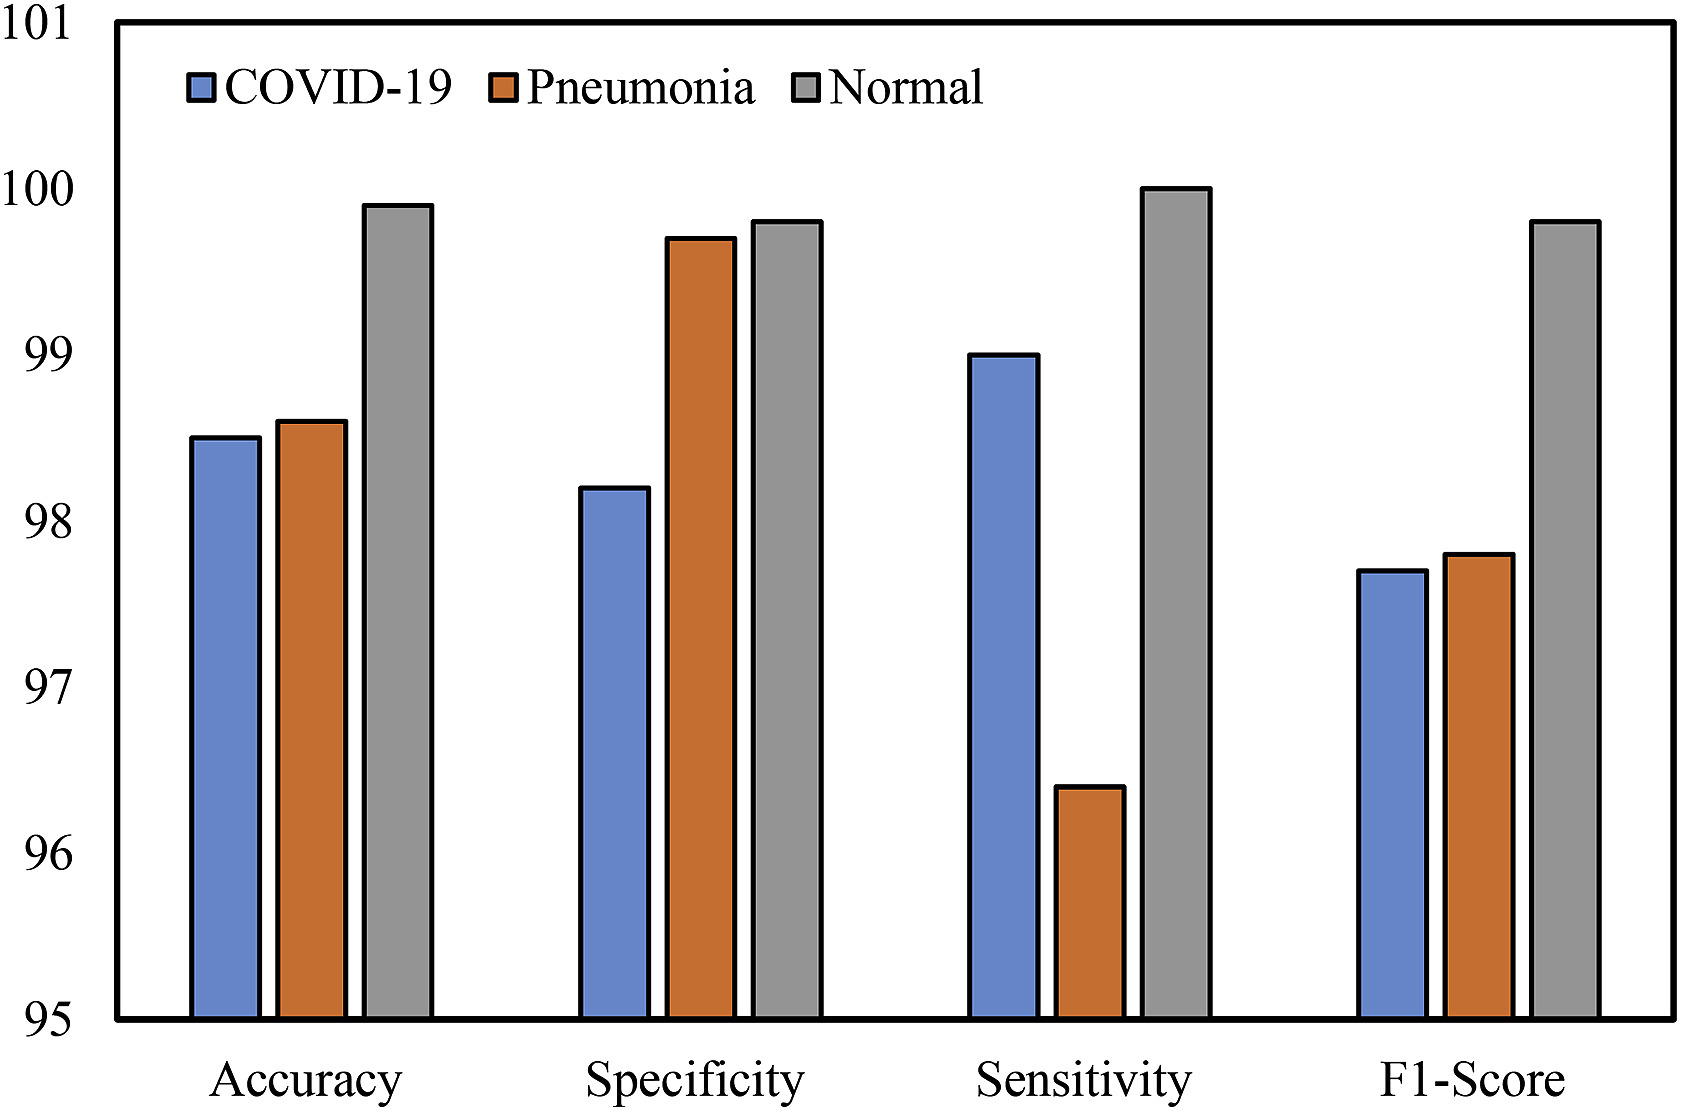
\includegraphics[width=1\textwidth,height=0.5\textheight]{Images/performanceOfCNN-LSTMPaper.png}
    \caption{Perfomance of CNN model\cite{litReviewCnnLstm}}
    \label{fig:Performance of CNN Model Literature Review}
\end{figure}
Figure \ref{fig:Performance of CNN Model Literature Review} shows the performance of a standard CNN model the accuracy ratings are as follows:
\begin{table}[h]
    \centering
    \begin{tabular}{|c|c|c|c|c|}
    \hline
         Class
         & Accuracy
         & Specificity
         & Sensitivity
         & F1-Score\\
         \hline
         COVID-19 & 98.5 &  98.2 & 99.0 & 97.7 \\
         Pneumonia & 98.6 & 99.7 & 96.4 & 97.8 \\
         Normal & 99.9 & 99.8 & 100.0 & 99.8\\
         \hline
    \end{tabular}
    \caption{Results of Standard CNN Network - A combined deep CNN-LSTM network for the detection of COVID-19 using X-ray images}
    \label{tab:Results of CNN - A combined deep CNN-LSTM network for the detection of COVID-19 using X-ray images}
\end{table}
\vspace{0.5mm}
 \begin{figure}[H]
    \centering
    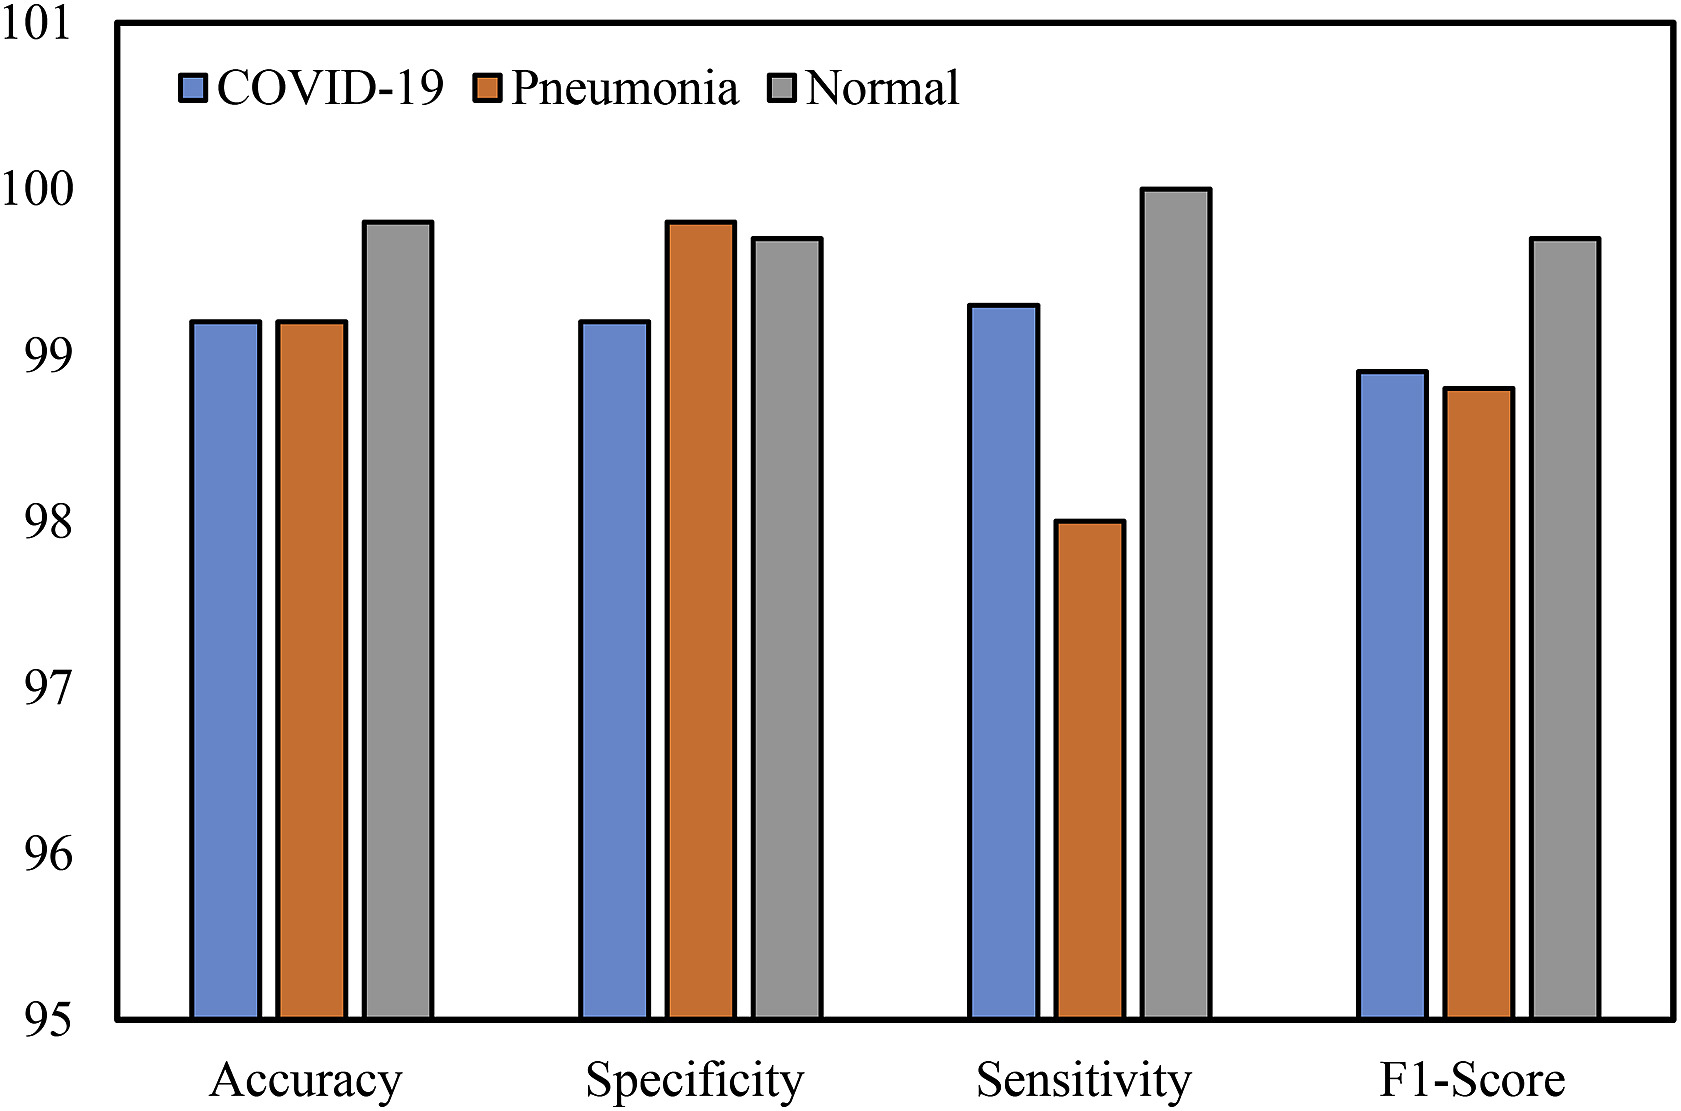
\includegraphics[width=1\textwidth,height=0.5\textheight]{Images/performanceOfCNNLSTM-LSTMPaper.png}\\
    \caption{Performance of CNN LSTM Model\cite{litReviewCnnLstm}}
    \label{fig:Performance of CNN LSTM Model Literature Review}
\end{figure}
\vspace{0.5mm}
\begin{table}[h]
    \centering
    \begin{tabular}{|c|c|c|c|c|}
    \hline
         Class
         & Accuracy
         & Specificity
         & Sensitivity
         & F1-Score\\
         \hline
         COVID-19 & 99.2 &  99.2 & 99.3 & 98.9 \\
         Pneumonia & 99.2 & 99.8 & 98.0 & 98.8 \\
         Normal & 99.8 & 99.7 & 100.0 & 99.7\\
         \hline
    \end{tabular}
    \caption{Results of CNN - A combined deep CNN-LSTM network for the detection of COVID-19 using X-ray images}
    \label{tab:Results of CNN LSTM - A combined deep CNN-LSTM network for the detection of novel coronavirus (COVID-19) using X-ray images}
\end{table}
From figure \ref{fig:Performance of CNN LSTM Model Literature Review} it is clear that the model utilizing LSTM outperformed the basic CNN model on almost all fronts (with the exception of classification of normal patients which experienced a small decrease in accuracy), yielding a higher accuracy, specificity, sensitivity and F1 score for identifying COVID-19, and Pneumonia from X-rays.
\\
Despite the results achieved by the model, the final model suffers from lack of data which the researchers address in the conclusion section of this paper.  The other shortcoming of this model is that it focuses on posterior-anterior view of X-Rays meaning that it cannot diagnose X-Rays which are in other formats.  The authors of the paper also address that X-Rays, where the patient is afflicted with multiple diseases, cannot be efficiently classified by the model and the model's accuracy was not compared with that of radiologists.  Data augmentation may prove useful for such a model using a combination of CNN and LSTM.
\\
\section{Challenges \& Limitations of Using Artificial Intelligence in Automated Diagnosis Systems for COVID-19}
In a paper by Huang,Yang and others, researchers offer an analysis of the challenges of developing Artificial Intelligence to assist medical professionals in the identification and diagnosis of COVID-19.  As mentioned previously in this thesis the challenges include: lack of data, lack of data quality and the use of poorly merged data sets termed as Frankenstein data sets when training models. There are, however, more challenges that are faced when developing diagnostics tools, as discussed in the previously cited paper\cite{litReviewCnnLstm} it is very difficult to find people who are COVID-19 positive and asymptomatic due to them not getting treatment as no symptoms are apparent.  The labelling of data is also an issue as the X-rays of patients may only show moderate signs of COVID-19 which yields a risk of mislabelled data by clinicians.  There is also a risk of false positives and false negatives when developing a diagnostic tool.  False positives would cause a patient to unnecessarily be quarantined and false negatives could cause a patient to inadvertently spread COVID-19 to others.  Some patients who have already been infected with the virus may show no signs on CT images which also yield high false negative rates making it difficult to distinguish COVID positive patients from COVID negative patients.  
\\
To mitigate these challenges the researchers suggest that when developing an Artificially Intelligent diagnostic system the developer should combine chest imaging, exposure history and laboratory tests when training and testing the model.  Such data, however, is hard to come by as there are multiple laws concerning data-collection and ethical questions regarding the patient's right to privacy.   
\section{Research into Data Augmentation And Convolutional Neural Networks Architectures}
Data augmentation allows artificial intelligence researchers to artificially inflate the size of the amount of data, this is done by utilizing existing data and detecting patterns in the data.  From the original data, new data is produced using various methods such as rotating images, applying filters, altering various aspects of the image (such as padding, cropping, and zooming), etc. There are numerous techniques and methodologies for using data augmentation but for the purpose of this thesis we will be using Generative Adversarial Networks to create new data\ref{fig:Example GAN Diagram} for the purpose of improving upon existing automated diagnostic models for COVID-19.  There are multiple different types of GAN architecture that have been covered in the introduction section of this thesis.  The key advantages of using data augmentation are as follows: larger training set to train models on,  reduces overfitting, helps to prevent underfitting and improve the accuracy of the model, reduces the cost / time associated with the collection of new data, and increases the the trained model's ability to generalize.  There are however some challenges when it comes to using data augmentation such as: inability to reduce bias of new data(if there is bias in the existing data the new data will also contain bias), hard to generate discrete data such as text, and the data generated will need to be evaluated.
\\
In a paper by Tanaka and Aranha\cite{litReviewGanDataAugmentation} the researchers outline two algorithms to oversample the minority class within the data with the aim of balancing the data set.  These two methodologies are called SMOTE (Synthetic Minority Over-sampling Technique)\cite{litReviewSmote} and ADASYN (Adaptive Synthetic Sampling Approach for Imbalanced Learning)\cite{litReviewAdasyn}.  
\\
SMOTE works by creating artificial data which takes into account the data's position, a random point in the least represented class in the dataset is selected and SMOTE identifies members of the same class within the data by using the $k$-nearest neighbour algorithm which is a form of unsupervised learning.  SMOTE then generates an entirely new point in the vector for each pair which is situated between the two pieces of data, the new point is then positioned at a random percentage away from the initial point chosen.\cite{litReviewGanDataAugmentation}
\vspace{0.5mm}
 \begin{figure}[H]
    \centering
    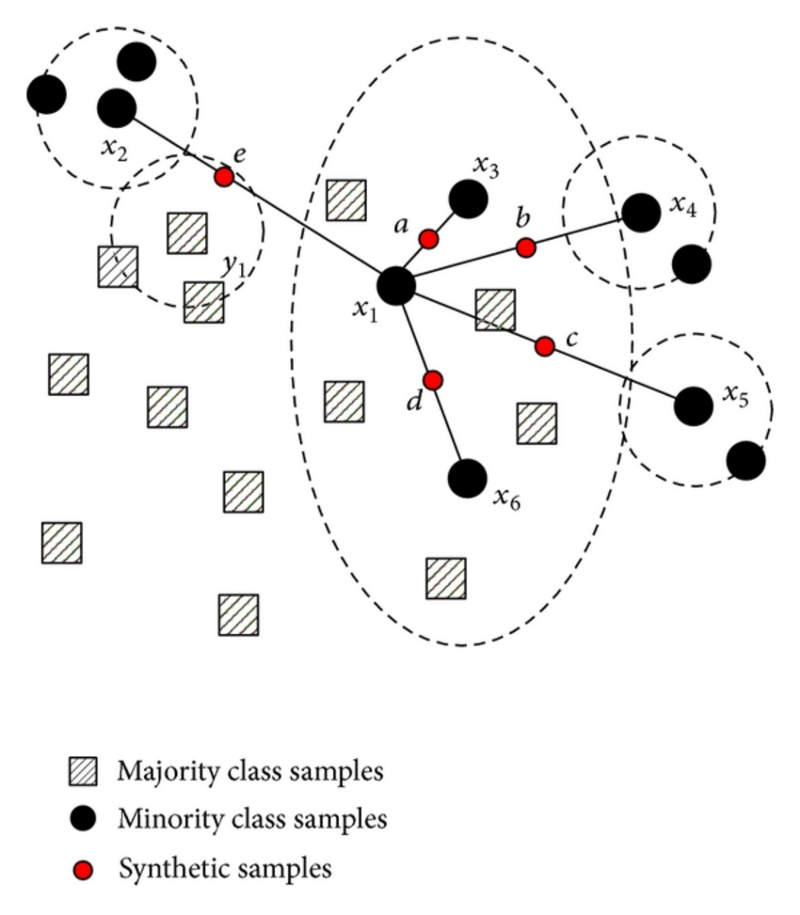
\includegraphics[width=1\textwidth,height=10cm,keepaspectratio]{Images/SMOTE.png}\\
    \caption{Example of SMOTE\cite{litReviewSmote}}
    \label{fig:Example of The SMOTE Algorithm}
\end{figure}
\vspace{0.5mm}
As we can see from figure\ref{fig:Example of The SMOTE Algorithm} the algorithm functions by detecting points between minority class samples, the points being determined by the $k$-nearest neighbour algorithm.  This ensures that the newly generated data will be similar to the already existing data of the minority class.  This may prove useful when developing the Generative Adversarial Network to create synthetic COVID-19 X-Rays.
\\
ADASYN works in a similar way to SMOTE and was originally based on SMOTE.  Both function in much the same way but the key difference lies in ADASYN adding a random small bias value to the points, breaking linear correlation to their parents.  The bias that ADASYN adds helps to increase the amount of variance within the synthetic data.  In this research paper the authors decided to evaluate the performance of the GANs ability to generate synthetic numerical data in two domains, one domain is concerned with training a classifier which was trained only using synthetic data and the other domain to created a balanced data set by oversampling the minority class using synthetic data.  The first domain's performance was measured by comparing the overall performance of the classifier on the original dataset with the overall performance of the classifier on the synthetic data set which were created by variations in the GAN architecture.  The researchers gauged the performance of the second domain by comparing the clasifier's performance on an imbalanced dataset oversampled with a standard GAN, SMOTE, and ADASYN as well as the original data set which is not oversampled.  SMOTE and ADASYN produce desirable results but the drawback is that they do not generalize well with sparse data and outliers according to the researchers.
\\
In both experimental domains, the researchers used the following GAN architecture to generate the synthetic data:
\begin{itemize}
    \item Leaky ReLU as activation function with a negative slope of 0.2
    \item batch size of 5
    \item learning rate of 2$\times10^{-4}$
    \item use of dropout in the GAN generator with a probability of 0.3
    \item Binary cross-entropy as loss function
    \item Adam as the optimizer
    \item No convolution layers
    \item If the generator has more than one layer, they are ordered in ascending size
    \item In the discriminator, layers are ordered in descending size if there is more than 1 layer
\end{itemize}\cite{litReviewGanDataAugmentation}
They also used the following architectures to generate the data:
\begin{table}[H]
    \centering
    \begin{tabular}{|c|c|}
    \hline
         Data Set Name
         & Architecture of GAN\\
         \hline
         Original Data & The first 70\% of the original database\\
         256/512/1024 & Generated by a GAN with 3 hidden layers with size 256, 512 and 1024\\
         256/512 & Generated by a GAN with 2 hidden layers with size 256 and 512\\
         256 & Generated by a GAN with 1 hidden layer with size 256\\
         128/256/512 & Generated by a GAN with 3 hidden layers with size 128, 256 and 512\\
         128/256 & Generated by a GAN with 2 hidden layers with size 128 and 256\\
         128 & Generated by a GAN with 1 hidden layer with size 128\\
         \hline
    \end{tabular}
    \caption{GAN Architectures used for experiments in\cite{litReviewGanDataAugmentation})}
    \label{tab:GAN architecture(Data Augmentation using GANs paper)}
\end{table}
choices in the above architecture are standard within the literature in this area.  The performance of the GAN was then tested on 3 data sets which are listed below.
\begin{itemize}
    \item Pima Indians Diabetes data Database
    \item Breast Cancer Wisconsin Data Set (Diagnostic)
    \item Credit Card Fraud Detection
\end{itemize}
Using these data sets the researchers conducted a number of experiments to judge the performance of data augmentation when testing the classifier.  The first experiment involved the training of a classifier which was trained on synthetic data generated by the GAN.  The GAN was trained on the original data set for 1500 epochs. After training, the GAN was then used to generate synthetic data  containing the same amount of data as the original data set.  The classification label used by the GAN is a continuous value between 0 and 1, the value is then made discrete (either 0 or 1) which is determined by the process of rounding the integer to the nearest value.  The synthetic data generated was then utilized to train a classification tree and the tree was then tested by using a test subset which was created from the original data set. The GAN was trained using labeled class data also,  this allows the synthetic data to have any class and the GAN will determine of which class the data is a member.  Tests for experiment one were conducted on both the diabetes and cancer data sets, these data sets were not very unbalanced in terms of classes.  The findings of this experiment are visible in figure \ref{fig:Results from Experiment One(Data Augmentation Using GANs)} where the researchers compared classes in the newly generated synthetic data with data in the original data set.
\vspace{0.5mm}
 \begin{figure}[H]
    \centering
    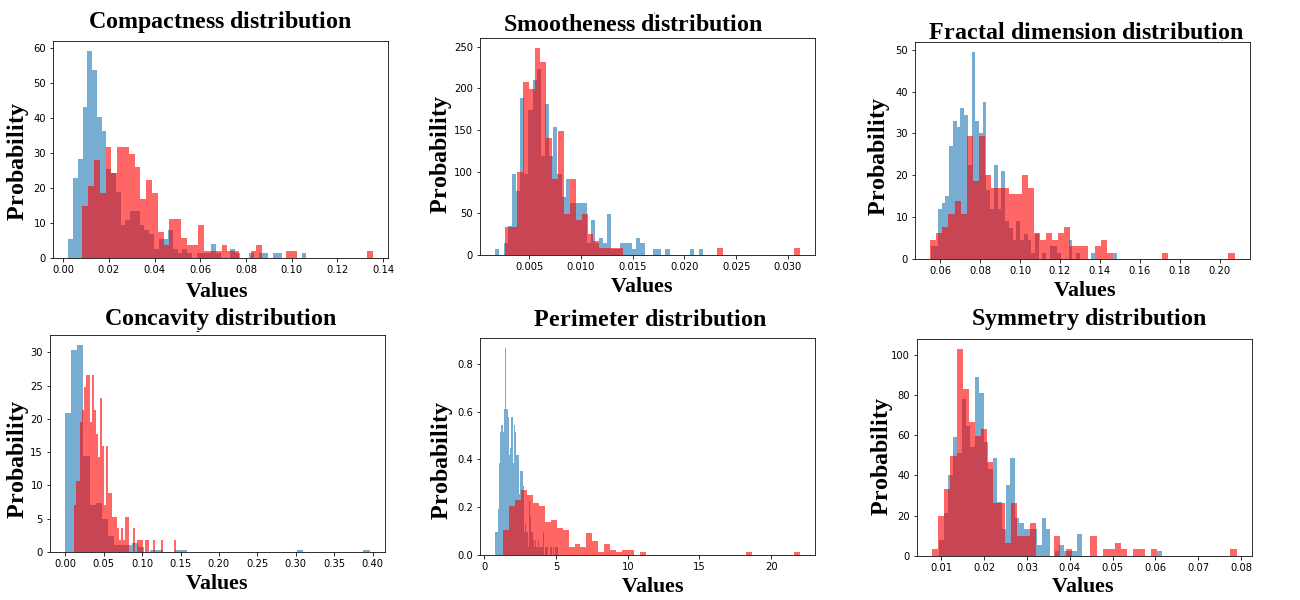
\includegraphics[width=1\textwidth,height=10cm,keepaspectratio]{Images/Experiment1GanDataAugmentation.png}\\
    \caption{Results from Experiment One (Data Augmentation Using GANs)\cite{litReviewGanDataAugmentation}}
    \label{fig:Results from Experiment One(Data Augmentation Using GANs)}
\end{figure}
\vspace{0.5mm}
The blue region in the image \ref{fig:Results from Experiment One(Data Augmentation Using GANs)} represents the distribution of features in the original data set where as the red represents the distribution of features in the newly created synthetic data. Figure \ref{fig:Results from Experiment One(Data Augmentation Using GANs)} shows that the synthetic data has a much more varied distribution.  From using the synthetic data the researchers were able to obtain the following results shown in table \ref{tab:Results and label distribution of Cancer Dataset using different GAN Architectures (Data Augmentation using GANs)}
\begin{table}[H]
    \centering
    \begin{tabular}{|c|c|c|}
    \hline
         Database
         & Label Proportion
         & Test Accuracy\\
    \hline
         Original Data Set & 56.53/43.47 & 0.888\\
         256/512/1024 & 52.26/47.74 & 0.818\\
         256/512 & 56.28/43.72 & 0.941\\
         256 & 56.78/43.22 & 0.906\\
         128/256/512 & 54.02/45.98 & 0.953\\
         128/256 & 58.04/41.96 & 0.935\\
         128 & 54.27/45.73 & 0.912\\
    \hline
    \end{tabular}
    \caption{Results of Cancer data set using different GAN Architectures Experiment 1 (Data Augmentation using GANs)\cite{litReviewGanDataAugmentation}}
    \label{tab:Results and label distribution of Cancer Dataset using different GAN Architectures (Data Augmentation using GANs)}
\end{table}
These results indicate that classifiers trained with the synthetic data generated by the various GAN architectures had superior results than the classifier trained with the original data set.  The only exception to this was the GAN with an architecture of 256/512/1024 which showed a small reduction in test accuracy.
\\
\begin{table}[H]
    \centering
    \begin{tabular}{|c|c|c|}
    \hline
     Database 
     & Label Proportion
     & Test Accuracy\\
     \hline
         Original Data Set & 64.8/35.2 & 0.748\\
         256/512/1024 & 71.69/28.31 & 0.7\\
         256/512 & 67.23/32.77 & 0.548\\
         256 & 67.6/32.4 & 0.748\\
         128/256/512 & 60.15/39.85 & 0.661\\
         128/256 & 65.18/34.82 & 0.739\\
         128 & 54.27/45.73 & 0.697\\
    \hline
    \end{tabular}
    \caption{Results and label distribution of Diabetes data set using different GAN Architectures Experiment 1 (Data Augmentation using GANs)\cite{litReviewGanDataAugmentation}}
    \label{tab:Results and label distribution of Diabetes Dataset using different GAN Architectures (Data Augmentation using GANs)}
\end{table}
The results of classifiers trained on the GAN architectures did not perform as well as those trained on the original data set when using the Diabetes data set.  As is shown from the table above the classifiers trained using synthetic data struggled to match the performance of classifiers trained with the original data set.  The GAN with the architecture of 1 hidden layer consisting of 256 units did manage to match the classifier trained on the original data set in terms of performance, the rationale for using the synthetic data would therefore be to increase the model's ability to generalise when encountering new data.
\\
In the second experiment conducted by the researchers, they tested the oversampling of the minority class in the data set by using both SMOTE and ADASYN.  The study proceeded as follows: The training set was separated based on the class of the target. The GANs were then trained only on minority-class data.  The GAN was then used to add new synthetic data to the data set thus increasing the number of instances of the minority class in the dataset, making this minority class more numerous within the data.  The researchers augmented the dataset with this new synthetic data creating new instances of the minority class until the data set was balanced. The synthetically augmented data set was then used when training a new classifier. The new classifier was then tested on both data sets, the original set, and the newly created synthetically augmented version which was created by allowing the majority class to be undersampled.
The results obtained from this experiment are shown in table \ref{tab:Classification results on imbalanced test set (Data Augmentation using GANs)}
\begin{table}[H]
    \centering
    \begin{tabular}{|c|c|c|c|}
         \hline
         Database
         & Accuracy
         & Precision 
         & Recall \\
         \hline
         Original & 0.999 & 0.896 & 0.556\\
         SMOTE & 0.958 & 0.026 & 0.861 \\
         ADASYN & 0.958 & 0.026 & 0.861 \\
         128 & 0.798 & 0.051 & 0.806 \\
         256 & 0.986 & 0.077 & 0.789 \\
         128 / 256 & 0.974 & 0.045 & 0.82 \\
         256 / 512 & 0.964 & 0.033 & 0.808\\
         \hline
    \end{tabular}
    \caption{Classification results on imbalanced test set experiment 2 (Data Augmentation using GANs)\cite{litReviewGanDataAugmentation}}
    \label{tab:Classification results on imbalanced test set (Data Augmentation using GANs)}
\end{table}

\begin{table}[H]
    \centering
    \begin{tabular}{|c|c|c|c|}
         \hline
         Database
         & Accuracy
         & Precision 
         & Recall \\
         \hline
         Original & 0.782 & 1.0 & 0.565\\
         SMOTE & 0.912 & 0.959 & 0.861 \\
         ADASYN & 0.921 & 0.979 & 0.861 \\
         128 & 0.807 & 0.89 & 0.806 \\
         256 & 0.894 & 0.998 & 0.789 \\
         128 / 256 & 0.902 & 0.981 & 0.82 \\
         256 / 512 & 0.888 & 0.962 & 0.808\\
         \hline
    \end{tabular}
    \caption{Classification results on balanced test set experiment 2 (Data Augmentation using GANs)\cite{litReviewGanDataAugmentation}}
    \label{tab:Classification results on balanced test set (Data Augmentation using GANs)}
\end{table}
It's clear from the tables above the use of SMOTE and ADASYN underperformed in accuracy on the imbalanced test set but had higher recall when compared with the original.  In the second table, when tested on the balanced test set, SMOTE and ADASYN outperformed the original in terms of accuracy and recall. This is due to the original data set being imbalanced, the tree trained on this data set predicts almost all samples as negative. The GAN using a hidden layer of 128 performed very poorly in both instances when compared with other GAN architectures and this is called out by the researchers in the paper.  Oversampling the minority seemed to increase the recall score of the classifier but at the expense of precision.  The results shown above will prove useful in guiding the development of the architecture used in the GANs to generate synthetic COVID data, and to over sample the minority of the classes within the various datasets I plan on using to train the classifier, this will be discussed further in later chapters.
\\
Through this research, the researchers found that when dealing with very unbalanced test sets, the GAN outperformed both SMOTE and ADASYN when it came to accuracy and precision but had a lower overall recall score.  Depending on the context of the problem domain accuracy and precision may be preferred over recall or recall may be preferred over accuracy and precision.
\\
When developing the GANs for generating synthetic data to train COVID-19 classifier, there are questions that will need to  be answered when deciding to use SMOTE and ADASYN over a traditional GAN architecture.  A higher accuracy and precision would be useful in diagnosing COVID-19 in all patients while reducing the risk of unnecessary quarantining due to false positives.  However, a higher recall would yield a higher overall identification of COVID positive patients but at the expense of precision, this would help to reduce the transmission of the virus but at the expense of causing unnecessary quarantines of patients.
 \\
There are a few limitations the researchers of this paper addressed in this study.  The research was conducted using only three data sets it is unclear if the results found in the paper will be similar when utilizing other data sets.  There are also many other considerations to take into account when using GANs, such as mislabelled data, the size of the dataset, amongst other factors which may influence the creation of the synthetic data.
\\
In another paper, by Wang and Xiao\cite{litReviewLychee} a convolutional neural network was employed in order to discern defects in harvested lychee fruit.  The data set used was then augmented with synthetic data generated with a GAN.  To train the classifier and the GAN, researchers created a data set of 3743 samples which were divided into 3 categories: mature, defects, and rot.  The data set created by the researchers suffered from an imbalance much like the data set in the paper previously discussed\cite{litReviewGanDataAugmentation}.  To address the imbalance within the data set the researchers used a transformer-based GAN to augment the data and create a more diverse and balanced data set which was used to train the classifier to classify the lychee fruit.  The researchers created a number of deep convolutional neural network models which incorporated a number of architectures such as: SSD-MobileNet V2, Faster RCNN-ResNet50, and Faster RCNN-Inception-ResNet V2.  The models were trained with different hyper-parameters to evaluate and contrast their performance.  The researchers found from the evaluations of the models that the data augmentation did in fact increase the performance of the classifiers.
\\
There is much need for automation within this particular domain as human fatigue can affect the classification of lychee fruit and incorrect classification of lychee is costly to businesses both in monetary terms and in terms of reputation.  This problem domain within artificial intelligence has been extensively studied, commonly used methods for detecting defects within fruit are: region growing method, minimum outer rectangle method, threshold segmentation, edge detection, $k$-mean clustering, and contour finding\cite{litReviewLychee}.  Recent progress made in the field of deep learning has demonstrated superior results in a wide range of computer vision tasks among other tasks.  Through the use of a DCNN the authors of this paper \cite{litReviewLychee} hope to show superior performance in comparison to traditional machine learning methods currently in use.
\\
The researchers decided to use samples of black leaf lychee which were purchased from the Jiangbei Fruit Wholesale Market in Huzhou city which is located in Guangdong, China when creating the data set, the black leaf lychee were purchased in batches of two.  The first batch contained 2042 mature lychees, which contained 1216 sample which had cracks but had no signs of rot.  To gather rot samples for the data set the researchers stored the 625 cracked lychee samples in an environment which was dry and they were stored at room-temperature so they rotted naturally as opposed to artificially.  495 additional samples were rotted and dried by being exposed to sunlight.  The second batch contained 865 lychees that were utilized as a test sample to ensure the tests were not biased.  The two batches of lychee were then stored in boxes alongside ice packs and shipped back to the researcher's lab to maintain the fruit's freshness while in transit.  Data diversity was accomplished by gathering lychee images at six locations in Huizhou College at various times, the images were also taken from different angles.  A total of 5014 images were collected for the data set by the researchers.
\\
When training the neural network the researchers synthetically augmented the dataset in an attempt to reduce the overall risk of overfitting the model and to improve the model's generalisation ability by exposing the model to a far larger dataset.  The training set was augmented with synthetic data generated by the GAN below is a table of the distribution of categories from the original data set which the researchers were using to train the model.
\begin{table}[H]
    \centering
    \resizebox{\columnwidth}{!}{\begin{tabular}{|c|c|c|c|c|c|c|}
         \hline
         Category
         & Original
         & Original Percentage 
         & Training
         & Test
         & Generated
         & Augmented Training set\\
         \hline
         Mature & 1648 & 44.03\% & 1298 & 350 & 102 & 1400\\
         Defects & 964 & 25.75\% & 800 & 164 & 600 & 1400 \\
         Rot & 1331 & 30.22\% & 896 & 235 & 504 & 1400 \\
         Total & 3743 & 100.00\% & 2994 & 749 & 1206 & 4200\\
         \hline
    \end{tabular}}
    \caption{Comparison of distribution of data augmented vs original(lychee Surface Defect Detection Based on Deep Convolutional
Neural Networks with GAN-Based Data Augmentation)\cite{litReviewLychee}}
    \label{tab:Comparison of distribution of data augmented vs original(lychee Surface Defect Detection Based on Deep Convolutional Neural Networks with GAN-Based Data Augmentation)}
\end{table}
As shown in the table above the augmented data offers a much more balanced dataset with all classes of lychee being represented in equal proportion.  Classifiers trained on the original dataset may have possibly created a model which would create a high bias for the most represented class of lychee in the dataset. 

 \begin{figure}[H]
    \centering
    \includegraphics[width=1\textwidth,height=15cm,keepaspectratio]{Images/lycheeGANSetup.PNG}\\
    \caption{Figure of learning framework for lychee Classification Model\cite{litReviewLychee}}
    \label{fig:Figure of learning framework for lychee Classification Model (lychee Surface Defect Detection Based on Deep Convolutional Neural Networks with GAN-Based Data Augmentation) }
\end{figure}
\vspace{0.5mm}
Figure \ref{fig:Figure of learning framework for lychee Classification Model (lychee Surface Defect Detection Based on Deep Convolutional Neural Networks with GAN-Based Data Augmentation) } shows the overall configuration of how the models for lychee surface defect detection were trained.  The original training set was used to train the GAN and from the newly augmented training set the DCNN models were trained to detect defects.  After the training of the DCNN models they were validated on a test set to compare each model's performance in an unbiased manner. 
\\ 
In this paper, the researchers decided to use a variation of GAN known as TransGAN.  This version of a GAN is based on  transformers and did not use convolutions.  This version of a GAN consisted of a transformer encoder which is made up of a "multi-head self-attention module stacked by a feed-forward multilayer perceptron"\cite{litReviewLychee}.  This version of a GAN has traditionally been used for natural language processing but has also found applications in computer vision.  In this version of a GAN the generator $G$ alongside the discriminator, $D$ are created using transformer encoder blocks.  TransGAN has a multi-stage mechanism that will adjust the image resolution by upscaling and downscaling the image accordingly to prevent excessive memory consumption.  There is also a grid self-attention module which is contained within the first partition,  this is used to reduce the computational load.  TransGAN has shown superior results in generative modeling and hence was adopted by the researchers.\cite{litReviewLychee}\cite{litReviewTransGanResults}

 \begin{figure}[H]
    \centering
    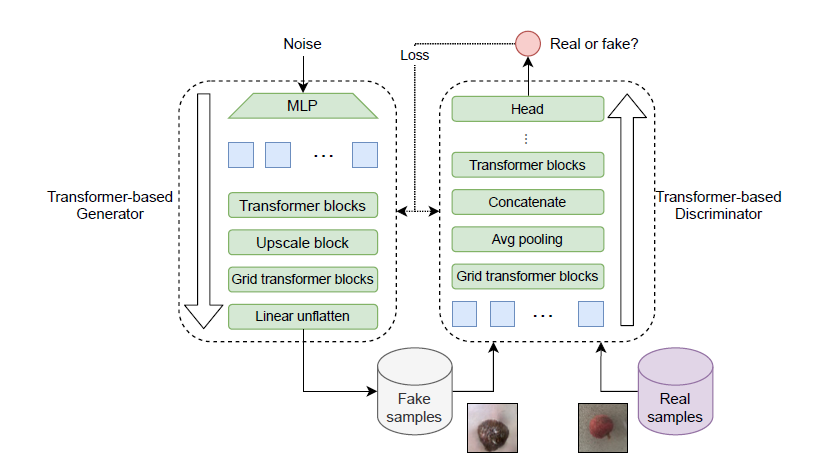
\includegraphics[width=1\textwidth,height=15cm,keepaspectratio]{Images/TransGan Figure.PNG}\\
    \caption{Figure of TransGAN (lychee Surface Defect Detection Based on Deep Convolutional Neural Networks with GAN-Based Data Augmentation)\cite{litReviewLychee}}
    \label{fig:Figure of TransGAN for lychee Classification Model (lychee Surface Defect Detection Based on Deep Convolutional Neural Networks with GAN-Based Data Augmentation)}
\end{figure}
\vspace{0.5mm}
%continue on from page 6
There are a variety of DCNNs used in this paper, we will show diagrams used by the researchers and explain each before further investigating the results of this paper as it's important to understand how each DCNN functions and compare each model's advantages and disadvantages.

 \begin{figure}[H]
    \centering
    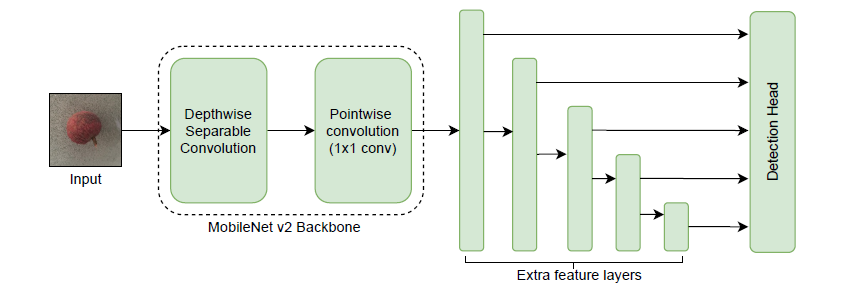
\includegraphics[width=1\textwidth,height=15cm,keepaspectratio]{Images/SSD-MobileNet V2 Architecture.PNG}\\
    \caption{Figure of SSD-MobileNet V2 Architecture (lychee Surface Defect Detection Based on Deep Convolutional Neural Networks with GAN-Based Data Augmentation)\cite{litReviewLychee}}
    \label{fig:Figure of SSD-MobileNet V2 Architecture for lychee Classification Model (lychee Surface Defect Detection Based on Deep Convolutional Neural Networks with GAN-Based Data Augmentation)}
\end{figure}
\vspace{0.5mm}
Figure \ref{fig:Figure of SSD-MobileNet V2 Architecture for lychee Classification Model (lychee Surface Defect Detection Based on Deep Convolutional Neural Networks with GAN-Based Data Augmentation)} shows an example of an SSD-MobileNet V2 DCNN as shown the input goes throw a depthwise separable convolution and a pointwise convolution.  The goal of SSD is to be able to perform object localization alongside object classification in only one forward pass of the network.  SSD uses multi-scale feature mapping which allows the neural network which mimics the human eye when detecting and classifying objects.  MobileNet is a lightweight deep neural network which has been identified as being efficient at performing a number of tasks.  The model consists of two hyper-parameters which include both, a  resolution multiplier, and a width multiplier. These hyperparameters can be tuned to yield a higher latency or a higher accuracy for speed.  Each convolutional layer uses both batch normalization alongside a ReLU activation function.  The original version of the MobileNet (V1) consisted of an input layer, 13 convolutional layers, an average pooling layer and a fully connected layer\cite{litReviewLychee}.  In MobileNetV2 two new features were added these included a bottleneck which is linear between each layer and a connection shortcut between bottlenecks in the model which allowed for more efficient training.  
 \begin{figure}[H]
    \centering
    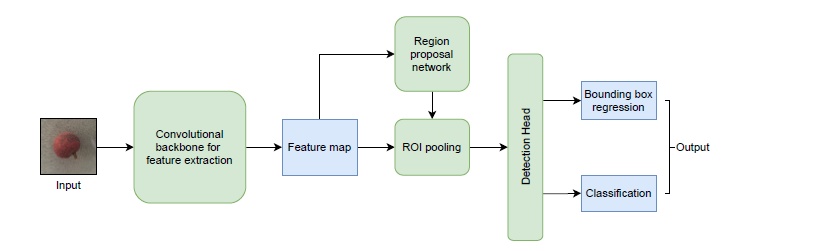
\includegraphics[width=1\textwidth,height=15cm,keepaspectratio]{Images/FasterRCNN.PNG}\\
    \caption{Figure of Faster RCNN Architecture (lychee Surface Defect Detection Based on Deep Convolutional Neural Networks with GAN-Based Data Augmentation)\cite{litReviewLychee}}
    \label{fig:Figure of Faster RCNN Architecture for lychee Classification Model (lychee Surface Defect Detection Based on Deep Convolutional Neural Networks with GAN-Based Data Augmentation) }
\end{figure}
\vspace{0.5mm}
Figure \ref{fig:Figure of Faster RCNN Architecture for lychee Classification Model (lychee Surface Defect Detection Based on Deep Convolutional Neural Networks with GAN-Based Data Augmentation) } shows the architecture of an RCNN-ResNet50 DCNN, this model was originally proposed by Girshick et al in a 2014 paper \cite{litReviewRCNN}.  This proposed DCNN model is utilized to perform search which is selective to extract 2000 regions from a given image, the regions extracted are termed as ``region proposals``\cite{litReviewRCNN}.  Candidate region proposals are converted into a square shape and then passed into a CNN that generates a 4096 dimensional feature vector, this feature vector is then input into an SVM(Support Vector Machine) to discern the data's classification.  This model is not suited for real time detection as the researchers found it took approximately 47 seconds to classify a single image, if using this architecture in the COVID-19 diagnostics CNN model there might possibly be a trade-off in terms of the time needed to classify data and the model's accuracy.  Due to the long time taken to classify an image, the researchers proposed a new architecture aptly termed ''Faster RCNN'' which would eliminate the selective search and instead input the entire image into the  CNN to produce the convolutional feature map.  This architecture  does not have to process 2000 proposals every time it classifies an image, which reduces the amount of time taken by the model to classify the image.
 \begin{figure}[H]
    \centering
    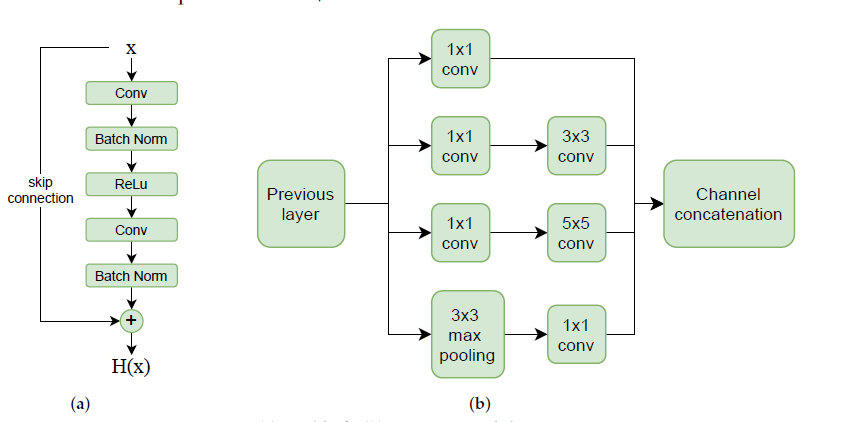
\includegraphics[width=1\textwidth,height=15cm,keepaspectratio]{Images/FasterRCNNResBlockInceptionModule.PNG}\\
    \caption{Figure of Faster RCNN Res Block and Inception Module (a) Res block; (b) Inception Module. (lychee Surface Defect Detection Based on Deep Convolutional Neural Networks with GAN-Based Data Augmentation)\cite{litReviewLychee}}
    \label{fig:Figure of Faster RCNN Res Block and Inception Module (lychee Surface Defect Detection Based on Deep Convolutional Neural Networks with GAN-Based Data Augmentation)}
\end{figure}
\vspace{0.5mm}
The final model proposed by the researchers, aims to include an inception model to offer "superior local topology for the neural network"\cite{litReviewLychee}.  The module (b) which is shown in figure \ref{fig:Figure of Faster RCNN Res Block and Inception Module (lychee Surface Defect Detection Based on Deep Convolutional Neural Networks with GAN-Based Data Augmentation)} aims to perform several convolutional operations on the input image, each operation occurs in parallel, and combines all the results into a deep feature map.  The model uses a numerous array of different filters to perform such convolutional operations on the input and obtains an array of information about the image.  The methods used when designing this model allows for the model to gain a much deeper understanding of the image.
\\
The researchers used the following configuration to train the TransGAN to generate synthetic data
\begin{itemize}
    \item Learning rate of $1 \times 10 ^ {-4}$
    \item Adam as an optimizer
    \item batch size of 64 for both the generator and discriminator models
    \item The training ran for 220 epochs
\end{itemize}

The DCNNs were then trained on both the original and augmented training sets, training 6 different models in total.  Every model which was trained took an image as input and then showed a box over the image for each detected lychee along with a predicted category along with a score of how confident the model was in classifying the lychee.  The hyperparameter settings for each model were as follows:
\begin{itemize}
    \item Weight decay of $5 \times 10 ^{-4}$
    \item Momentum of $8 \times 10^{-1}$
    \item Verification Period of 5000
    \item Batch Size of 32
    \item Learning Rate of $5 \times 10^{-3}$
    \item And ran for a total of 1500 epochs
\end{itemize}

The results before augmentation for the models are shown in the table below \ref{tab:Results of models before Augmentation Lychee}
\begin{table}[H]
    \centering
    {\begin{tabular}{|c|c|}
         \hline
         Name of Model
         & Mean Average Precision\\
         \hline
         SSD-MobileNet V2 & 88.95\%\\
         Faster RCNN-ResNet50 V2 & 91.57\%\\
         Faster RCNN-Inception-ResNet V2 & 91.25\%\\
         \hline
        \end{tabular}}
    \caption{Results of models before Augmentation(lychee Surface Defect Detection Based on Deep Convolutional
Neural Networks with GAN-Based Data Augmentation)\cite{litReviewLychee}}
    \label{tab:Results of models before Augmentation Lychee}
\end{table}
The researchers found that training on the GAN-augmented data that the performance increased by the following amounts for each of the models.
\begin{table}[H]
    \centering
    {\begin{tabular}{|c|c|}
         \hline
         Name of Model
         & Performance Gain\\
         \hline
         SSD-MobileNet V2 & 2.86\%\\
         Faster RCNN-ResNet50 V2 & 1\%\\
         Faster RCNN-Inception-ResNet V2 & 0.58\%\\
         \hline
        \end{tabular}}
    \caption{Improvement of model's mean average precision after Augmentation(lychee Surface Defect Detection Based on Deep Convolutional
Neural Networks with GAN-Based Data Augmentation)\cite{litReviewLychee}}
    \label{tab:Improvement of model accuracy after Augmentation Lychee}
\end{table}
As we can see from the above table \ref{tab:Improvement of model accuracy after Augmentation Lychee} SSD-MobileNet V2 had the most gains in terms of performance.  Due to the large imbalance between classes in the dataset the performance gap is quite large.  The mean average precision performance gaps between classes before augmentation is shown in the table below \ref{tab: Mean average precision before Augmentation Lychee}
\begin{table}[H]
    \centering
    {\begin{tabular}{|c|c|}
         \hline
         Name of Model
         & Mean Average Precision Performance Gap\\
         \hline
         SSD-MobileNet V2 & 9.45\%\\
         Faster RCNN-ResNet50 V2 & 6.12\%\\
         Faster RCNN-Inception-ResNet V2 & 7.77\%\\
         \hline
        \end{tabular}}
    \caption{Mean average precision before Augmentation(lychee Surface Defect Detection Based on Deep Convolutional
Neural Networks with GAN-Based Data Augmentation)\cite{litReviewLychee}}
    \label{tab: Mean average precision before Augmentation Lychee}
\end{table}
After the augmentation process, the researchers found that the mean average precision performance gaps between classes were reduced for each of the three models to the values shown in table \ref{tab: Mean average precision after Augmentation Lychee}
\begin{table}[H]
    \centering
    {\begin{tabular}{|c|c|}
         \hline
         Name of Model
         & Mean Average Precision Performance Gap\\
         \hline
         SSD-MobileNet V2 & 1.78\%\\
         Faster RCNN-ResNet50 V2 & 4.45\%\\
         Faster RCNN-Inception-ResNet V2 &  2.35\%\\
         \hline
        \end{tabular}}
    \caption{Mean average precision after Augmentation(lychee Surface Defect Detection Based on Deep Convolutional
Neural Networks with GAN-Based Data Augmentation)\cite{litReviewLychee}}
    \label{tab: Mean average precision after Augmentation Lychee}
\end{table}
As we can see from the above values the augmentation process yielded better quality models that can better differentiate between the three classes of fruit (rotten, defective, and mature).  The model which has shown the most improvement in terms of mean average precision was Faster RCNN-ResNet50, however the researchers found that Faster
RCNN-Inception-ResNet V2 was the most accurate in detecting rotten samples.
 \begin{figure}[H]
    \centering
    \includegraphics[width=1\textwidth,height=15cm,keepaspectratio]{Images/MeanAvgPrecisionlychee.png}\\
    \caption{Figure of Mean Average Precision of Models. (lychee Surface Defect Detection Based on Deep Convolutional Neural Networks with GAN-Based Data Augmentation)\cite{litReviewLychee}}
    \label{fig:Figure of Mean Average Precision of models (lychee Surface Defect Detection Based on Deep Convolutional Neural Networks with GAN-Based Data Augmentation) }
\end{figure}
Given that detecting defects in lychee is a time-sensitive job the researchers compared each of the three models in terms of detection speed.  This is also a significant factor when developing the diagnostic models for detecting COVID-19 as the sooner the virus can be detected the sooner it can be treated effectively.
 \begin{figure}[H]
    \centering
    \includegraphics[width=1\textwidth,height=15cm,keepaspectratio]{Images/AnalysisofModelSpeedlychee.png}\\
    \caption{Figure of Speed of Models in classifying lychee. (lychee Surface Defect Detection Based on Deep Convolutional Neural Networks with GAN-Based Data Augmentation)\cite{litReviewLychee}}
    \label{fig:Figure of Speed of Models in classifying lychee (lychee Surface Defect Detection Based on Deep Convolutional Neural Networks with GAN-Based Data Augmentation) }
\end{figure}
As we can see above SSD-MobileNet V2 classifies the lychee faster than the other two models although all 3 models met the researcher's requirement for lychee defect detection.  These results are of particular interest and may prove useful when designing the automated diagnosis tool for COVID-19.  SSD-MobileNet V2 could perhaps diagnose the patients faster than the medical professionals analyzing the patient, thus freeing up time for medical professionals to assist other patients.
\\
I will list the accuracy of each of the models with and without data augmentation below to compare and contrast the classification performance.
\begin{table}[H]
    \centering
    \resizebox{\columnwidth}{!}{\begin{tabular}{|c|c|c|c|c|c|}
         \hline
         Model
         & Setting
         & Acc 
         & Rec
         & Spe
         & F1\\
         \hline
         SSD-MobileNet V2 & Base setting & 89.81\% & 90.08\%&89.89\%&89.46\%\\
         SSD-MobileNet V2 & GAN Augmentation & 91.96\% & 92.06\%&91.99\%&91.92\%\\
         \hline
         Faster RCNN-ResNet50 & Base Setting & 91.82\% & 92.23\%&91.95\%&91.72\%\\
         Faster RCNN-ResNet50 & GAN Augmentation & 92.76\% & 92.96\%&92.80\%&92.55\%\\
         \hline
         Faster RCNN-Inception-ResNet V2 & Base Setting & 91.96\% & 92.07\%&91.98\%&91.54\%\\
         Faster RCNN-Inception-ResNet V2 & GAN Augmentation & 92.36\%  &91.74\%& 92.22\%& 91.86\%\\
         \hline
        \end{tabular}}
    \caption{Comparison of accuracy of base models vs models with data augmentation(lychee Surface Defect Detection Based on Deep Convolutional
Neural Networks with GAN-Based Data Augmentation)\cite{litReviewLychee}}
    \label{tab:Comparison of accuracy of base models vs models with data augmentation(lychee Surface Defect Detection Based on Deep Convolutional Neural Networks with GAN-Based Data Augmentation)}
\end{table}
As shown in the above table \ref{tab:Comparison of accuracy of base models vs models with data augmentation(lychee Surface Defect Detection Based on Deep Convolutional Neural Networks with GAN-Based Data Augmentation)} all of the models had better accuracy, recall(with the exception of Faster RCNN Inception model), specificity and F1 score with the data augmented data set.  This shows that the classifiers were more accurate when classifying the fruit when they were trained on a more balanced data set.
\section{Conclusion}

From analyzing existing models for the automated detection of COVID-19 it appears that data quality and data shortage are key areas where improvements could be made to improve the overall accuracy and usability of the existing models.  From the analysis of the current paradigms in convolutional neural networks and data augmentation of this thesis it is clearly shown that data augmentation has proven very useful in a wide range of applications which range from detecting defects in lychee to  identifying credit card fraud.  Given the positive results shown in the given problem domains, it seems a reasonable conjecture that the use of data augmentation would also prove useful for COVID-19 detection.  In the next sections of this thesis, I will discuss the implementation methods used when creating both the convolutional models and the data augmentation models, the results of the models implemented, and further research which could be conducted into this area.  It will be interesting to see if the findings of the papers explored above are transferable to this new problem domain.